% !TEX TS-program = pdflatex
% !TEX encoding = UTF-8 Unicode

%************************************************
\chapter{La Performance}
\label{chp:La Performance}
%************************************************

\begin{quotation}
Since music began to be notated, clearer distinctions between the work and its performance, and between the composer and performer, have emerged, representing multifarious views of the role of the performer.\footnote{Tanja Orning \textit{Pression} (a performance study) Norwegian Academy of MusicMusic Performance Research Copyright © 2012 Royal Northern College of Music Vol. 5}
\end{quotation}

Introduco questo paragrafo con una citazione estrapolata da un articolo scritto da Tanja Orning su \textit{Pression} di Helmut Lachenmann. La semplicità con la quale il compositore è riuscito a trasformare il gesto in scrittura è di grande interesse. Infatti, è una grande intuizione l'unione di una notazione standard fusa assieme a disegni rappresentanti gesti precisi sullo strumento. Come vediamo in fig. \ref{fig:lach}, ogni linea è connessa ad un determinato movimento sullo strumento: facile da recepire e intuitivo nell'esecuzione. 

\begin{figure}[htbp]
\begin{center}
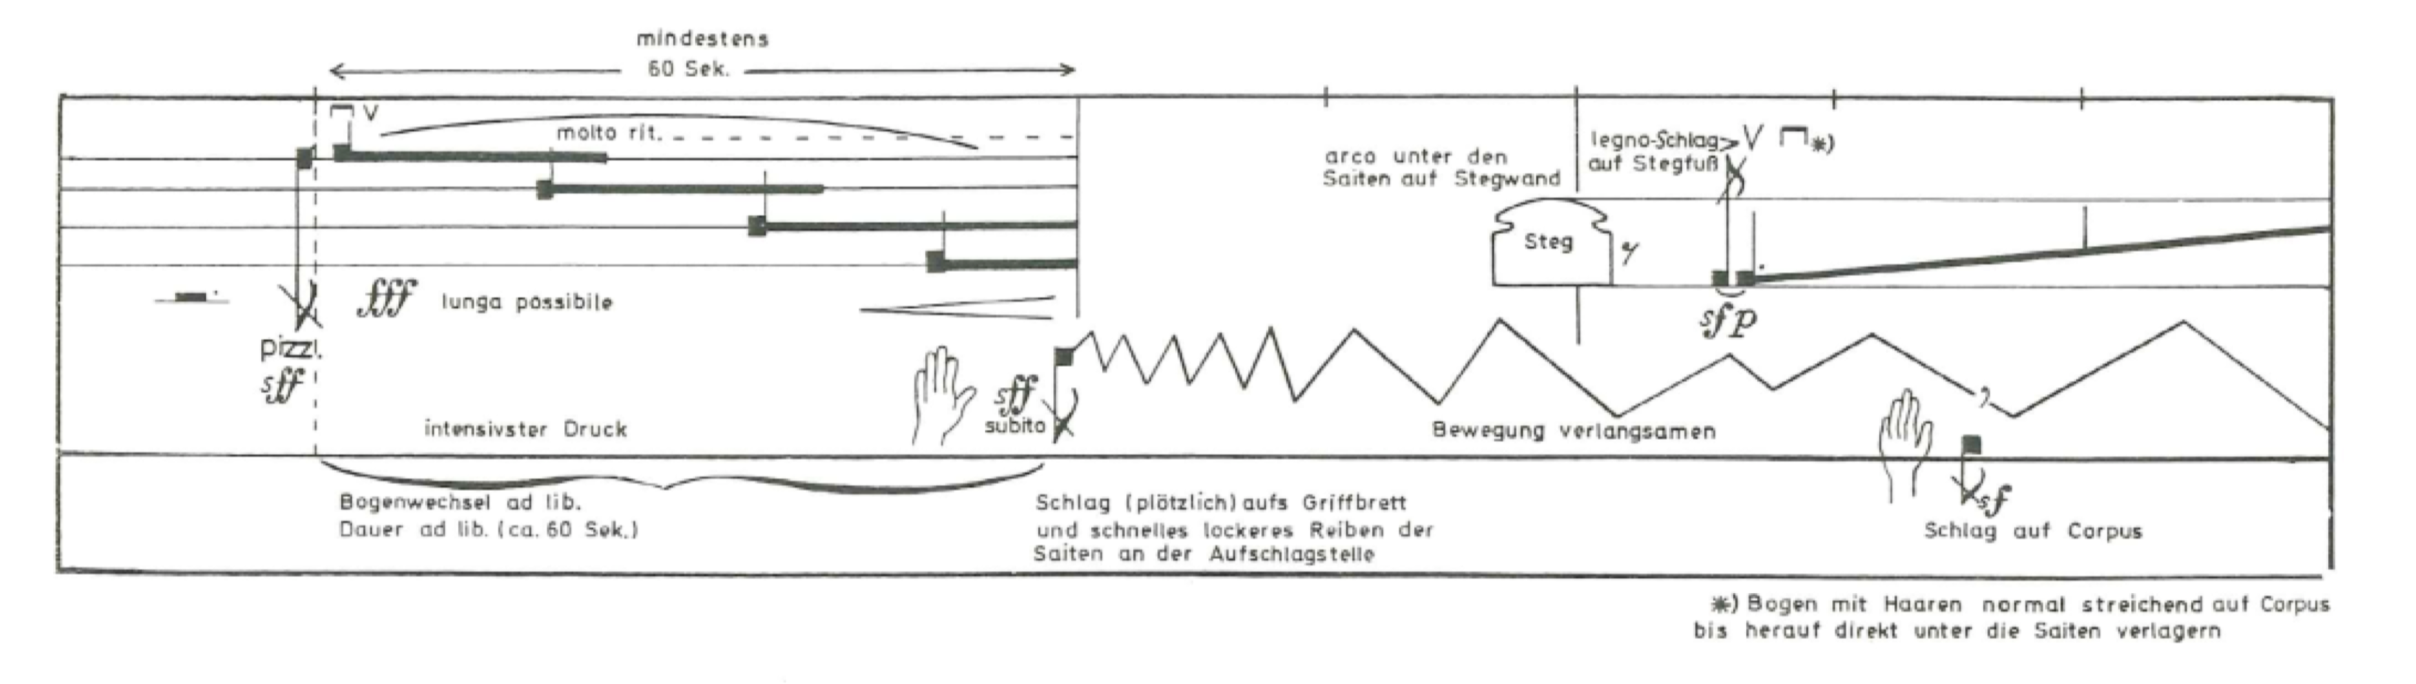
\includegraphics[width=1.\textwidth]{Lachenmann02.jpg}
\caption{particolare partitura \textit{Pression}}
\label{fig:lach02}
\end{center}
\end{figure}

Penso che il lavoro da fare sulla performance, parta proprio da questa base e le riflessioni da fare, vertono su tre punti principali:

\begin{itemize}
\item{Dialogo tra performer e compositore. Ogni consiglio deve essere ben accetto così da rendere l'ultima stesura della partitura chiara e vicina alle esigenze dello strumentista. Più si matura e più si raggiunge una maggiore intelligibilità.}
\item{La presenza di gesti legati alla fisicità dello strumento e ad un legame tra movimento e simbologia.}
\item{Immaginare sia i gesti che l'andamento formale onde evitare refusi e impossibilità fisiche performative.}
\end{itemize}

%************************************************

\section{Legame tra esecutore, performer e \newline compositore}

\epigraph{Non si tratta di opprimere il pubblico con preoccupazioni cosmiche trascendenti. Che possano esservi chiavi profonde del pensiero e dell'azione in base alle quali leggere tutto lo spettacolo[...].
Tuttavia è necessario che queste chiavi esistano; e la cosa riguarda noi}{Antonin Artaud \\ Il teatro e il suo doppio}

Trovo affascinante il modo in cui i musicisti approcciano al loro strumento e ogni strumentista lo fa in modo diverso e intimo. 

Studiando tecniche estese ho sempre subito questa fascinazione e mi ritrovo ripetutamente a modificare le mie partiture e l'approccio con i musicisti a volte risulta complicato. La questione è che, considero la stesura della partitura, come un tramite per conoscersi ed interagire con chi la esegue. Ecco perché, mi capita spesso di rimettere mano ai miei spartiti per far sentire a proprio agio il performer. Matteo Fracassi, studente del dipartimento di percussioni del Santa Cecilia, si è prestato a questo esperimento e ha deciso di intraprendere un percorso conoscitivo addentrandosi nelle maglie della mia scrittura.

Il lavoro fatto su Sp.I.R.E. è stato leggermente diverso da quelli svolti in passato, perché essendo un nuovo strumento, ogni approccio non aveva riferimenti precedenti. Si sono riscontrare delle difficoltà prima di tutto di scrittura: ogni gesto doveva essere rappresentato da un simbolo e soprattutto ogni timbro doveva legarsi ad una dinamica, una durata e ad un pitch (anche se non definito). Inoltre, avendo cinque molle e quattro placche non si può utilizzare una notazione standard, composta da uno spartito classico. Sicuramente, la notazione metronomica e l'utilizzo di accenti facilita la performance, così da dare risalto alle micro-forme interne e alla struttura del pezzo.

Un altro problema legato all'esecuzione è il contenuto timbrico e la dinamica dei gesti. Nell'approccio ad un nuovo strumento, non sempre le dinamiche hanno la stessa scala di valori tra chi le scrive e chi le legge, è opportuno infatti riportare degli esempi e se necessario suonarli noi stessi all'interprete. In alcuni casi è buono solfeggiare assieme delle parti. Ogni miglioramento richiesto dallo strumentista va valutato e prontamente segnato per poi riportarlo in partitura. Un apporto essenziale del percussionista è stato nella stesura della partitura base: l'utilizzo di colori differenti per le placche e le molle, la diminuzione in un rigo unico per ogni molla o placca e l'aggiunta del cambio di battente, sono tutte caratteristiche aggiunte dopo svariati colloqui con Fracassi. 

Tutto si può migliorare e semplificare per facilitare l'esecuzione ed eliminare i refusi. L'interprete/performer si deve dedicare esclusivamente all'interpretazione del flusso formale. Inoltre, Il legame tra gesto e figura è strettamente correlato. Ogni gesto avrà bisogno di un riscontro sonoro per evitare che l'ammaliante timbrica di Sp.I.R.E. porti a rapportarcisi in modo più improvvisativo che di studio. In pratica, ogni gesto rappresentato in partitura sarà la risultante sonora di un determinato timbro o di un determinato armonico.

Il performer, quindi, deve possedere una capacità performativa estesa alla conformazione dello strumento,  deve avere la capacità di seguire una struttura compositiva salda e oltremodo precisa. Allo stesso modo, riuscire a districarsi nella lettura di una scrittura a tratti, libera. Il performer deve saper unire tra loro i fraseggi che si incastrano, si restringono e si dilatano nel tempo (durata delle frasi) e nello spazio (estensione dello strumento) mantenendo un ictus costante che dia un'identità formale alla composizione.
